\subsection{Baby \& Mother's Health}
The baby's and mother's health is an important factor during and after childbirth. Successful childbirth often depends on some key factors of the baby's health such as gestational age, the weight of the baby when it was born, etc. To analyze this we looked into the Australian dataset (figure \ref{fig:bmi_au}) and we can observe that the majority of the babies were underweight at the time they were born. It can often happen as sometimes doctors suggest mothers be conservative about eating during the last stage of pregnancy as the labour can become very difficult if the baby is overweight \emph{[citation needed]}.
\begin{figure}
  \centering
  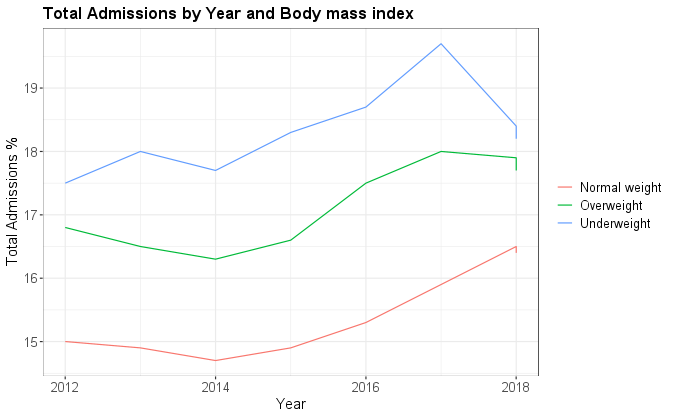
\includegraphics[width=0.75\textwidth]{subsections/baby_health/bmi.png}
  \caption{BMI of babies in Australia over the years.}
  \label{fig:bmi_au}
\end{figure}
Below are the findings we get after analysing data that focuses on ACT data only.

\subsubsection{Gestational Age of Babies in ACT}
Gestational age refers to the amount of time a fetus has spent in the womb, starting from the first day of the mother's last menstrual period. It is typically measured in weeks and is used to track fetal development and monitor the progress of pregnancy.

Babies born between 37 and 40 weeks are considered full-term and are generally at a lower risk for complications than those born earlier. These babies have had enough time to develop and mature in the womb, which can help ensure that they are able to breathe, eat, and maintain their body temperature after birth.

Babies born before 37 weeks are considered premature and may require special care and monitoring in a neonatal intensive care unit (NICU). Premature babies are at a higher risk for a range of complications, including respiratory distress syndrome, jaundice, and infections.

On the other hand, babies born after 40 weeks are considered post-term and may also be at a higher risk for complications, such as macrosomia (large birth weight), meconium aspiration syndrome, and fetal distress. In these cases, medical professionals may recommend inducing labor to ensure the health and safety of both the mother and the baby.

\begin{figure}
  \centering
  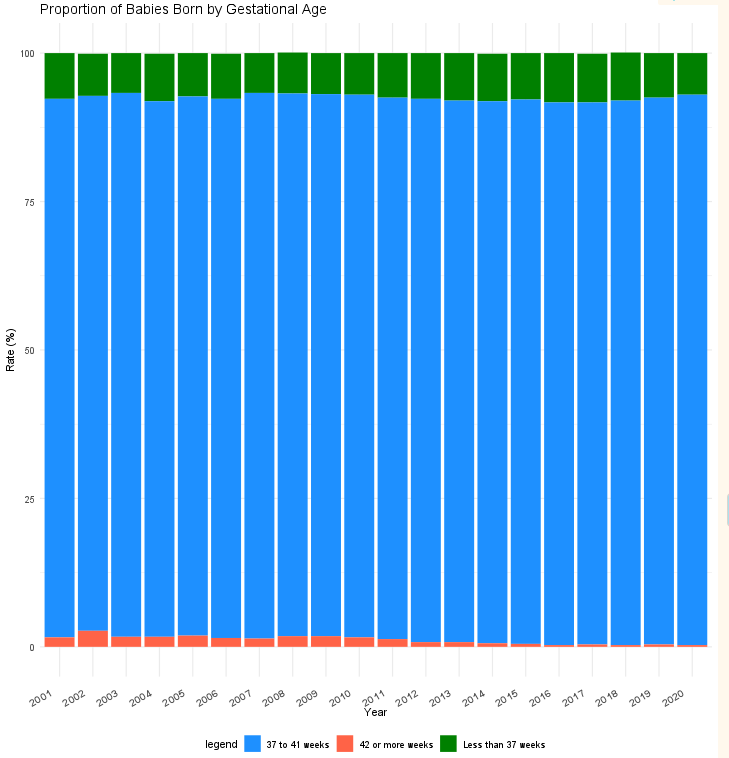
\includegraphics[width=0.8\textwidth]{subsections/baby_health/gestational_age_act.png}
  \caption{Gestational age of babies in ACT.}
  \label{fig:gest_act}
\end{figure}

In \textbf{Figure \ref{fig:gest_act}} we can see that the gestational age of babies has been really good which is over 90\%.
\subsubsection{Underweight Newborn of Babies in ACT}
Ideally, a baby is considered underweight if its weight is less than 2500 grams. In order to determine how ACT is doing in this regard we generated a visualization that shows the percentage of babies who are underweight grouped by their gestational age \textbf{(figure \ref{fig:weight_gest})}. We can see that most of the underweight babies born are from the ideal gestational period. This may seem misleading but can be explained if we look at \textbf{figure \ref{fig:gest_act}} we can see that 90\% of the babies are born in that group which explains the disproportionate amount of babies in ACT being born underweight.

\begin{figure}
  \centering
  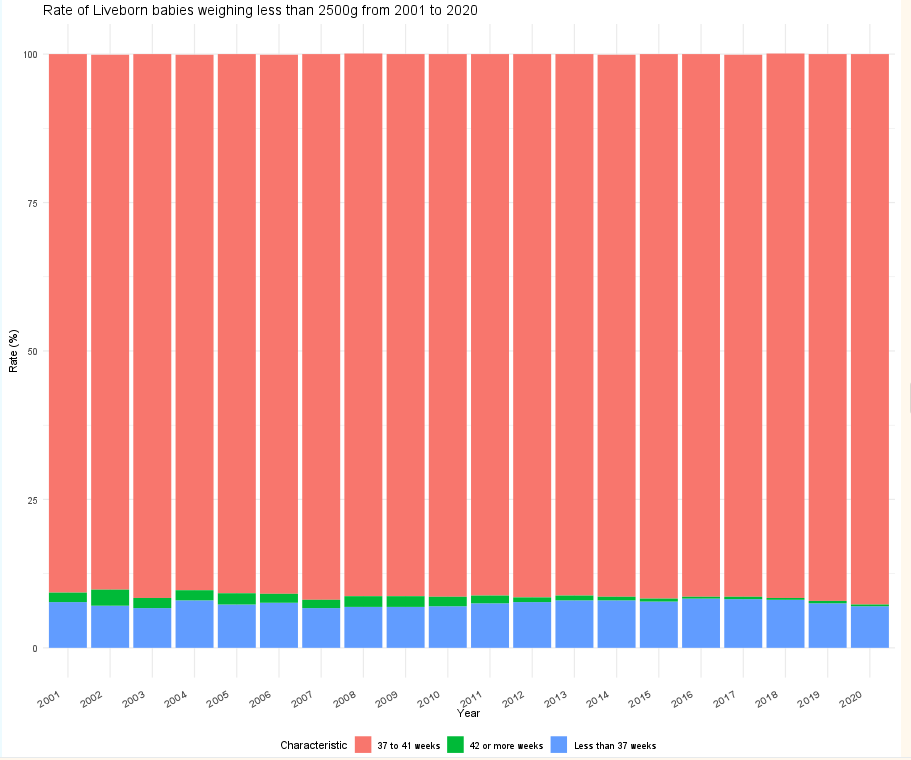
\includegraphics[width=0.8\textwidth]{subsections/baby_health/live_born_weigh_proportion_act.png}
  \caption{Liveborn baby weight proportion in ACT.}
  \label{fig:weight_gest}
\end{figure}

In \textbf{Figure \ref{fig:weight_act}} we can also see that even though the rate of underweight babies is around 5\% through the years it is showing an upward trend.

\begin{figure}
  \centering
  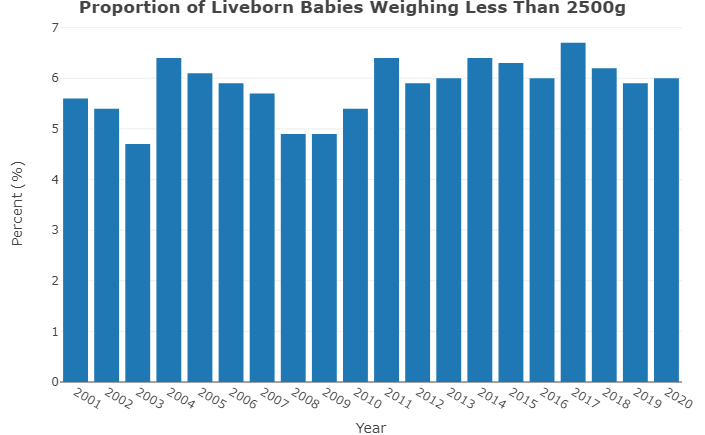
\includegraphics[width=0.8\textwidth]{subsections/baby_health/liveborn_weight.png}
  \caption{Underweight babies weight}
  \label{fig:weight_act}
\end{figure}
\subsubsection{Mother's Gestational Diabetes}
Gestational diabetes is a type of diabetes that occurs during pregnancy. It affects about 2-10\% of pregnant women and usually develops in the second or third trimester of pregnancy. Gestational diabetes can increase the risk of complications during pregnancy and delivery, as well as the risk of developing type 2 diabetes later in life.

The exact cause of gestational diabetes is not fully understood, but it is thought to be related to hormonal changes that occur during pregnancy. During pregnancy, the placenta produces hormones that can interfere with the body's ability to use insulin effectively. Insulin is a hormone that regulates blood sugar levels, and when the body is unable to use insulin properly, blood sugar levels can become elevated, leading to gestational diabetes.

Women who are at increased risk of developing gestational diabetes include those who are overweight or obese, have a family history of diabetes, have previously had gestational diabetes, have polycystic ovary syndrome (PCOS), or are older than 25 years of age.

Treatment for gestational diabetes usually involves dietary changes, such as reducing the intake of simple sugars and increasing the intake of complex carbohydrates, as well as regular exercise. In some cases, insulin injections may also be needed to control blood sugar levels. It is important for women with gestational diabetes to monitor their blood sugar levels regularly and attend all prenatal appointments to ensure that both they and their babies are healthy.

In \textbf{figure \ref{fig:gest_diabetes}} we can see a sudden spike in gestational diabetes among mothers in ACT.

\begin{figure}
  \centering
  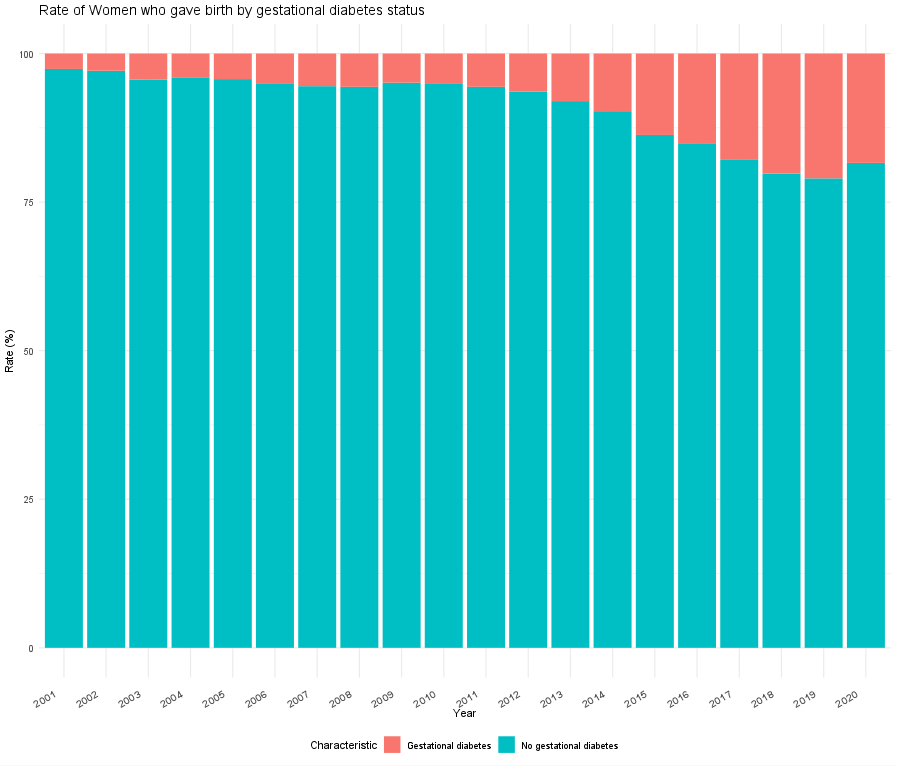
\includegraphics[width=0.90\textwidth]{subsections/baby_health/gestational_diabetes_rate.png}
  \caption{Gestational diabetes rate of mothers in ACT.}
  \label{fig:gest_diabetes}
\end{figure}